\documentclass[FisicaTeorica.tex]{subfiles}
\begin{document}
\chapter{Motivazione del formalismo}
\lesson{1}{01/10/2018}
Lo scopo del corso è comprendere il formalismo della meccanica quantistica basandosi sulle conoscenze acquisite in fisica moderna di come i concetti si siano sviluppati storicamente, ed imparare ad operare su sistemi quantistici elementari. La meccanica quantistica mette in crisi concetti come l’onda e la particella, le osservabili come la posizione ed il momento, la misura e lo stesso concetto di “realtà fisica”. Anche se risulta una teoria controintuitiva (se guardata in chiave classica) senza di essa il mondo risulterebbe inspiegabile (si pensi a fenomeni come l’incompenetrabilità dei corpi, stabilità della materia ecc...). I fenomeni quantistici, meno evidenti di quelli classici ma altrettanto reali, sono conseguenze delle proprietà del mondo macroscopico come descritto dalla meccanica quantistica. Inoltre l’elettronica moderna senza meccanica quantistica risulterebbe impossibile, dunque la meccanica quantistica ha diversi risvolti anche sulla tecnologia. \\
Per motivare il \textbf{formalismo} che sarà utilizzato nelle prossime lezioni, esaminiamo qualitativamente due fenomeni peculiari che manifestano l'incompatibilità tra mondo classico e quantistico: l'interferenza degli elettroni e la misura di polarizzazione dei fotoni.

\section{Interferenza degli elettroni}
Sparando degli elettroni \textbf{uno alla volta} contro due fenditure\index{Esperimento delle due fenditure}, dietro le quali viene posto uno schermo rivelatore, osserviamo i seguenti fenomeni:
\begin{enumerate}[label=\Roman*.]
    \item Sullo schermo \marginpar{Comportamento particellare} compare sempre un numero intero di $e^-$ (come se fossero particelle).
\end{enumerate}
Con due fenditure aperte otteniamo una figura interferenza per il numero di elettroni rilevati sullo schermo alla posizione $x$, dato da $N_{12}(x)$. Tale figura scompare se chiudiamo una delle due fenditure, e in tal caso si osserva un picco in prossimità della fenditura rimasta aperta. Chiamiamo $N_1(x)$ e $N_2(x)$ le misurazioni eseguite in questi due casi.\\
\begin{enumerate}[label=\Roman*.]
\setcounter{enumi}{1}
    \item Si ha che \marginpar{Comportamento ondulatorio} $N_{12}(x) \neq N_1(x) + N_2(x)$, o, equivalentemente, dividendo per $N$ (n. degli $e^-$) per ottenere delle probabilità, $p_{12}(x) \neq p_1(x) + p_2(x)$. In altre parole, la probabilità di trovare in $x$ un elettrone quando entrambe le fenditure sono aperte \emph{non} è la somma delle probabilità che si hanno nei due casi in cui solo una delle due fenditure è aperta.
\end{enumerate}
\marginpar{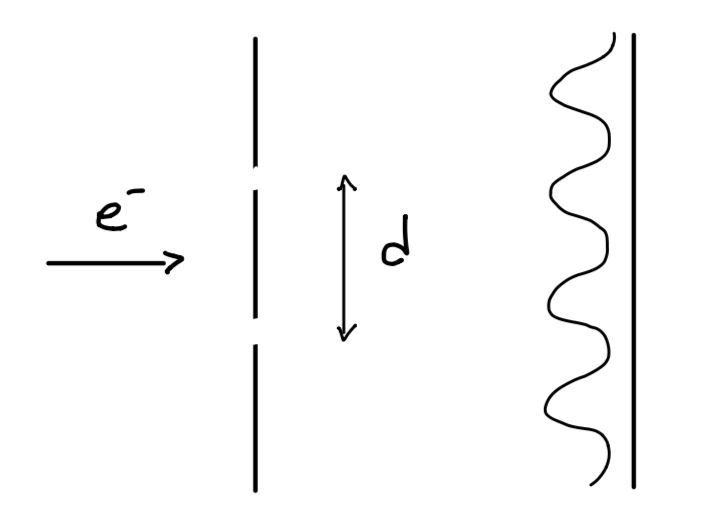
\includegraphics[width=3.5cm]{Immagini/interferenzafenditure.png}}

Possiamo interpretare I e II utilizzando una funzione d'onda $\psi(x)$ complessa, introdotta da Schrödinger e interpretata in maniera probabilistica da Born. Il modulo quadro $|\psi(x)|^2$ dà infatti la \textbf{densità di probabilità} di trovare l'elettrone in posizione $x$.\\
In questo modo è soddisfatta I, e anche II, in quanto, analogamente alle onde:
\[
\psi_{12}(x) = \psi_1(x) + \psi_2(x) \Rightarrow p_{12}(x) = |\psi_{12}(x)|^2 \neq |\psi_1(x)|^2 + |\psi_2(x)|^2 = p_1(x) + p_2(x)
\]
Perciò gli elettroni sono \q{particelle} la cui probabilità di essere trovate con una misura in una data posizione $x$ è data dal modulo quadrato della funzione d'onda $\psi(x)$.\\
Tale descrizione, seppur funzionale, è di difficile \q{intuizione fisica}. Per esempio, potremmo stimare la \q{lunghezza} di un elettrone $e^-$ tramite la sua lunghezza d'onda Compton $\lambda = \hbar/(mc) \approx 10^{-12} \, \mathrm{m}$. Ci aspettiamo che l'elettrone \q{conosca} il mondo esterno a questa scala. Ma una figura di interferenza compare anche quando la distanza tra le fenditure è molto maggiore, sulla scala di $10^{-5} \, \mathrm{m}$. Come può l'elettrone, giunto in prossimità di una fenditura, \q{sapere} se l'altra è aperta o meno ed eventualmente \q{produrre} la figura di interferenza?

Per ogni singolo elettrone è possibile determinare da \textit{quale} delle due fenditure è passato, per esempio predisponendo un sistema di illuminazione al di là della fenditura, che segnali il suo eventuale passaggio. Modificando così l'apparato sperimentale, tuttavia, la figura di interferenza scompare, e si ha che $N_{12}^\text{ill} = N_1(x) + N_2(x)$, e quindi $p_{12}^\text{ill} = p_1(x) + p_2(x)$.\\
Il formalismo deve quindi anche spiegare che:
\begin{enumerate}[label=\Roman*.]
\setcounter{enumi}{2}
    \item La possibilità \marginpar{L'atto di misura modifica il comportamento delle particelle} di conoscere la posizione \textit{intermedia} di una particella ne modifica il comportamento
\end{enumerate}

La spiegazione \q{euristica} di questa situazione è che la luce è composta da particelle quantistiche, i fotoni, e quando questi urtano gli elettroni liberi (effetto Compton) li disturbano\footnote{Rimane aperta la questione: come è possibile che questo \q{disturbo} sia esattamente tale da ricostruire la situazione classica, e cioè da rendere $p_{12}(x) = p_1(x) + p_2(x)$} modificandone l'impulso.\\
Se la luce fosse fatta di onde potremmo ridurre il disturbo riducendo l'intensità dell'onda, ma se osservo l'elettrone vuol dire che un fotone l'ha colpito (e quindi si sta comportando come particella).\\
Possiamo allora minimizzare l'effetto riducendo il momento del $\gamma$, ma così facendo, per de Broglie, $p = h / \lambda$, e quindi ridurre $p$ significa aumentare la lunghezza d'onda $\lambda$, e così si perde l'informazione su quale fenditura è stata utilizzata per passare. Sperimentalmente, quando $\lambda$ del fotone usato per l'illuminazione è dell'ordine della distanza tra le fenditure, gli elettroni \q{non sono disturbati} e producono la figura di interferenza.\\
Come vedremo, questa \q{spiegazione} non è completamente soddisfacente, ma almeno salva la meccanica quantistica da un problema di autoconsistenza.\\
Infatti, senza la doppia natura ondulatorio-corpuscolare delle particelle coinvolte i fenomeni descritti non sarebbero possibili.\\
Notiamo che per gli elettroni con funzione d'onda
$\psi_{12}(x) = \psi_1(x) + \psi_2(x)$
nessuna delle seguenti affermazioni è corretta:
\begin{enumerate}
    \item L'elettrone passa dalle fenditure 1 o 2.\\
    Esclusa perché $p_{12}(x) \neq p_1(x) + p_2(x)$.
    \item L'elettrone passa da entrambe le fenditure.\\
    Esclusa perché se cerchiamo di verificare da quale fenditura è passato la troviamo in una sola (e non appena lo sappiamo l'interferenza scompare).
    \item L'elettrone arriva allo schermo senza passare dalle fenditure.\\ Falsa, poiché se chiudiamo le fenditure non arrivano elettroni allo schermo.
\end{enumerate}
Da queste considerazioni vediamo che non è affatto ovvio poter assumere che l'elettrone \q{abbia} una posizione (intesa come un valore numerico) se non lo osserviamo, ma solo che lo troviamo in una posizione (come valore) se eseguiamo una misura, con una probabilità determinata da $\psi_{12}(x)$.


Possiamo rendere più preciso il concetto di \q{disturbo}. 
Se conosciamo la posizione ad un istante introduciamo un'indeterminazione nel momento (allo stesso istante), e di conseguenza, con l'evoluzione temporale, anche un'indeterminazione nelle posizioni agli istanti successivi.\\
Es. camera a nebbia: ogni \q{punto} visibile è dato dall'interazione tra una particella e una delle goccioline nella camera, e costituisce una misurazione (affetta da incertezza) della sua posizione, che introduce un'indeterminazione in quelle successive. Perciò alla fine non si misura la traiettoria effettiva della particella, ma una successione di punti non completamente \q{allineati lungo una curva}.
In ogni caso non è considerabile una traiettoria, in quanto per le indeterminazioni non è possibile capire cosa succede tra un punto e l'altro.\\
Possiamo riassumere ciò in un altro punto che deve essere soddisfatto dal formalismo utilizzato:
\begin{enumerate}[label=\Roman*.]
\setcounter{enumi}{3}
    \item È impossibile\index{Indeterminazione di Schrödinger} \marginpar{Principio di indeterminazione di Heisenberg}  determinare simultaneamente posizione e momento di una particella quantistica con precisione maggiore di  per il prodotto delle indeterminazioni. 
\end{enumerate}

Scopo della prima parte del corso sarà costruire un formalismo matematico consistente che sia in grado di spiegare le proprietà da I a IV o l'analogo per la polarizzazione dei fotoni che ora discutiamo.\\

\section{Polarizzazione dei fotoni} 
\index{Polarizzazione}Lo stato dell'elettrone nell'esempio precedente è descritto da una funzione d'onda $\psi(x)$, elemento di uno spazio vettoriale infinito-dimensionale (tipico delle onde).\\
Esistono tuttavia sistemi quantistici con spazi degli stati finito-dimensionali.\\
Un esempio istruttivo e familiare nella sua versione classica è quello che descrive la \textbf{polarizzazione} di un'onda elettromagnetica, classicamente, e dei fotoni che la compongono, quantisticamente.\\
Seguendo Dirac, partendo dal comportamento classico delle onde polarizzate con $N\gg 1$ fotoni, cercheremo di estrapolare il comportamento quantistico del singolo fotone.\\

Un'onda elettromagnetica classica \textit{piana} ideale (estensione infinita), di pulsazione $\omega = 2\pi/T$ e vettore d'onda di modulo $k = \omega/c$ che punta lungo la direzione di propagazione $\hat{z}$, è data da un campo elettromagnetico oscillante:
\[
\begin{cases}
E_x(\vec{x},t) = \op{Re}(E_{0x} e^{i(kz-\omega t + \alpha_x)}) = E_{0x}\cos(kz-\omega t+\alpha_x)\\
E_y(\vec{x},t) = \op{Re}(E_{0y} e^{i(kz-\omega t + \alpha_y)}) = E_{0y}\cos(kz-\omega t+\alpha_y)\\
E_z(\vec{x},t) = 0\\
c \vec{B}(\vec{x},t) = \hat{z} \times \vec{E}(\vec{x},t)
\end{cases}
\]
con $E_{0x}$ e $E_{0y}$ positivi, costanti e indipendenti da $\vec{x}$ e $t$, e $\alpha_x$, $\alpha_y$ sono parametri che regolano la \textit{fase} dei rispettivi campi.\\
\lesson{2}{03/10/2018}
Unendo l'informazione su intensità e fase lungo gli assi $x$ e $y$ (che è l'unica necessaria per definire la polarizzazione dell'onda) definiamo $E_j = E_{0j} e^{i\alpha_j} \in \bb{C}$. Perciò $E_x$ e $E_y$ così definiti (complessi) sono le due componenti del vettore \marginpar{Vettore di polarizzazione} polarizzazione $\psi$:
\[
\begin{pmatrix}
\psi_x\\ \psi_y
\end{pmatrix} = \begin{pmatrix}
E_x\\
E_y
\end{pmatrix}
\]
che d'ora in poi indicheremo seguendo la notazione di Dirac come $\ket{\psi}$. La polarizzazione di un'onda gioca un ruolo analogo alla posizione (data tramite la funzione d'onda) di una particella.\\
Analizziamo meglio $\ket{\psi}$. Sappiamo che un'onda che ha una \textit{polarizzazione lineare} \marginpar{Polarizzazione lineare}di angolo $\alpha$ rispetto a $\hat{x}$ può essere vista come la sovrapposizione di due onde di \textit{stessa fase} che hanno polarizzazioni lungo $\hat{x}$ e $\hat{y}$. Se l'onda iniziale ha ampiezza $E_0$, le due onde \q{proiettate} avranno ampiezza $E_{0x} = E_0\cos\alpha$ e $E_{0y} = E_0\sin\alpha$.\\ %Inserire figura pag. 511 Mencuccini
Perciò le polarizzazioni \q{possono essere sovrapposte},\marginpar{$\ket{\psi}\in \bb{C}^2$} cioè sommate, e quindi $\ket{\psi}$ è un elemento di uno spazio vettoriale complesso, che sarà isomorfo a $\bb{C}^2$ in quanto $\ket{\psi}$ è definito da due coordinate complesse.\\
\textbf{Nota:} Abbiamo scelto di utilizzare le coordinate in $\bb{C}$ per includere in $E_x$ e $E_y$ anche l'informazione sullo sfasamento. Per esempio, la sovrapposizione di due onde di polarizzazione ortogonale ma \textit{sfasate} di $\pi/2$ produce la \textit{polarizzazione ellittica}\marginpar{Polarizzazione ellittica}.\\
Data questa premessa, possiamo utilizzare per $\ket{\psi}$ gli \q{strumenti} disponibili su $\bb{C}^2$. Per esempio su $\bb{C}^2$ è definito un prodotto scalare, che denotiamo, seguendo la notazione di Dirac, come $\braket{ \cdot |  \cdot }$, cioè: $\braket{\phi|\psi} = \phi_x^* \psi_x + \phi_y^* \psi_y$, con $\bra{\phi}$ il funzionale lineare su $\bb{C}^2$ dato da $\bra{\phi}: \ket{\psi} \to \braket{\phi|\psi} \in \bb{C}$.\\
Notiamo quindi che il vettore $\ket{\psi}$ contiene informazioni ridondanti. In particolare non ci serve sapere il modulo del campo elettrico - ci interessa solo la direzione di oscillazione. Perciò potremmo fissarlo a $1$, imponendo: \marginpar{I riduzione di $\bb{C}^2$}
\[
\norm{\vec{E}} = \sqrt{|E_x|^2 + |E_y|^2} = 1
\]
Scegliamo quindi $\ket{\psi}$ tale che $\braket{\psi|\psi} = 1$ (norma unitaria).\\
Agendo \marginpar{Esempi di polarizzazione}nella base canonica di $\bb{C}^2$, alcuni esempi di diverse polarizzazioni (e relativi vettori) sono:
\begin{itemize}
    \item \textbf{Polarizzazione lineare}, che può essere lungo $\hat{x}$ se $\ket\psi = \ket{x} \equiv (1,0)^t$, oppure lungo $\hat{y}$ se $\ket\psi = \ket{y}\equiv (0,1)^t$. Oppure può avere, ad esempio, una polarizzazione a $45^\circ$ rispetto a $\hat{x}$ se $\ket\psi = \ket{45^\circ} = \frac{1}{\sqrt{2}}(\ket{x}+\ket{y})^t$;
    \item \textbf{Polarizzazione circolare}, che può essere destrorsa se $\ket\psi = \ket{R} = \frac{1}{\sqrt{2}}(1,i)$, oppure sinistrorsa se $\ket\psi = \ket{L} = \frac{1}{\sqrt{2}}(1,-i)^t$.
\end{itemize}
In realtà imporre $\norm{\psi} = 1$ per rimuovere informazioni ridondanti restringe lo spazio considerato da $\bb{C}^2$ a $\frac{\bb{C}^2\setminus\{0\}}{\bb{R}_+} \cong S^3$.\\
Matematicamente,\index{Spazio quoziente} questo è uno \textit{spazio vettoriale quoziente},\marginpar{Spazio vettoriale quoziente} ottenuto \q{identificando} tutti i punti che soddisfano una certa condizione, che in questo caso è \q{il differire solamente per un fattore di scala}. In maniera pittoresca lo spazio quoziente si può pensare (in questo caso) come il prodotto di \q{incollare} tra loro tutti i vettori che \q{puntano nella stessa direzione}, ma hanno diverse \q{lunghezze}. In tal modo si passa da una situazione (in $\bb{C}^2$) in cui ho infiniti modi di scrivere la stessa polarizzazione, a una (nello spazio quoziente) in cui ad ogni punto è associata una sola \q{direzione} di polarizzazione (non ancora una sola polarizzazione - c'è un'altra ambiguità da rimuovere che tratteremo tra poco).\\
Formalizziamo quanto appena detto in termini matematici.
\marginpar{Relazione di equivalenza} La \q{condizione} è data da una \textit{relazione di equivalenza}. Detti $x,y\in I$, con $I$ un insieme qualsiasi, una relazione di equivalenza, indicata con $x\sim y$, è una qualsiasi condizione che sia \textit{riflessiva} (se $x\sim x$ sempre), \textit{simmetrica} (se $x\sim y$ allora $y\sim x$) e \textit{transitiva} (se $x\sim y$ e $y\sim z$ allora $x\sim z$).\\
Data una relazione di equivalenza su un insieme, si possono costruire le \textit{classi di equivalenza}, ossia i sottoinsiemi $[x] = \{y \in I | y\sim x\}$. L'insieme di tutte le classi di equivalenza è lo spazio quoziente stesso, indicato con $I/\sim$.\\
Nel nostro caso la relazione di equivalenza è data da $\bb{R}_+$ così definita:
\[
\ket{\phi} \sim \ket{\psi} \quad \Leftrightarrow \quad \frac{\ket{\psi}}{\norm{\psi}} = \frac{\ket{\phi}}{\norm{\phi}}
\]
\textbf{Nota}: dobbiamo rimuovere $0$ da $\bb{C}^2$, in quanto il vettore nullo non definisce alcuna polarizzazione. Se non lo facessimo, inoltre, la relazione di equivalenza non sarebbe ben definita, dato che dividiamo per la norma.\\
Possiamo poi specificare ogni classe di equivalenza prendendo un suo rappresentativo (ossia un suo elemento qualsiasi). Per convenienza prenderemo, per ogni classe \q{direzione dei vettori di $\bb{C}^2 \setminus \{0\}$}, l'unico vettori che \q{punta in quella direzione} che ha anche norma unitaria.\\
Fissando la norma a $1$ lo spazio è quindi ristretto dal seguente vincolo:
\[
|\psi_x|^2 + |\psi_y|^2 = 1 \quad \Rightarrow \quad (\op{Re}\psi_x)^2 + (\op{Im}\psi_x)^2 + (\op{Re}\psi_y)^2 + (\op{Im}\psi_y)^2 = 1
\]
Lo spazio risultante è perciò isomorfo a $S^3$, ossia a una $3$-sfera\footnote{Una $n$-sfera è definita come $S^{n}=\left\{x\in \mathbb {R} ^{n+1}:\left\|x\right\|=r\right\}$}.
%Cosa significa usare \bb{R}_+ come relazione di equivalenza? E S^1?
In realtà, anche fissando il modulo del campo elettrico, non c'è ancora una corrispondenza biunivoca tra le polarizzazioni \q{fisiche} e i vettori $\ket{\psi} \in (\bb{C}^2\setminus\{0\})/\bb{R}_+$. O meglio, c'è nel caso ci limitassimo solo alle polarizzazioni lineari, mentre per quelle \q{che ruotano} c'è ancora un'informazione ridondante: abbiamo specificato due fasi\marginpar{II riduzione} ($\alpha_x$ e $\alpha_y$), ma quella che conta è la loro differenza. Potremmo quindi fissare una delle due e specificare solamente l'altra.\\
Definendo un'opportuna relazione di equivalenza $S^1$ (dati due vettori $(E_x, E_y)$ e $(E_x', E_y')$, se $E_x'$ e $E_y'$ sono semplicemente la rotazione - sul piano complesso $\bb{C}$ - di $E_x$ e $E_y$, allora i due vettori sono equivalenti, poiché la \q{differenza di fase} è la stessa in entrambi\footnote{Matematicamente, $E_x = a e^{i\varphi}$, $E_y = b e^{i\varphi}$ sono equivalenti a $E_x' = a e^{i\varphi + \alpha}$, $E_y' = b e^{i\varphi + \alpha}$, per $\alpha \in S^1$, ossia $\alpha$ che va da $0$ a $2\pi$ per poi ripartire da $0$ e \q{continuare a girare}}), e\marginpar{Sfera di Bloch} considerando il rispettivo spazio quoziente che la incorpori (oltre a quella sulla norma): $\mathcal{S}_{\text{pol}} \cong (\bb{C}^2 \setminus \{0\})/(\bb{R}_+ \times S^1) \cong S^2$ otteniamo finalmente lo spazio delle polarizzazioni, detto \textbf{sfera di Bloch}\index{Sfera di Bloch}.\\
L'isomorfismo con $S^2$ si nota scrivendo il vincolo precedente:
\[
(\op{Re}\psi_x)^2 + (\op{Im}\psi_x)^2 + (\op{Re}\psi_y)^2 + (\op{Im}\psi_y)^2 = 1
\]
e fissando una fase, ponendo, per esempio, $\op{Im} \psi_x = 0$. Si ottiene così una forma del tipo $x^2 + y^2 + z^2 = 1$, corrispondente alla comune sfera in $\bb{R}^3$ (detta $S^2$).
%Inserire figura rotazione di $E_x$ e $E_y$ per dimostrare equivalenza
Un punto nella sfera di Bloch corrisponde ad una e una sola polarizzazione \q{fisica} di un fotone.\\
\textbf{Nota}: la sfera di Bloch \textbf{non} è uno spazio vettoriale! Per questo, nei conti che faremo, continueremo ad usare $\ket{\psi} \in \bb{C}^2$, nonostante essi contengano un sacco di informazione ridondante.\\

La coppia $\{\ket{x},\ket{y}\}$ \marginpar{Basi ON}costituisce una base ortonormale in $\bb{C}^2$, cioè un insieme di stati ortogonali ($\braket{x|y} = 0$) tra loro e normalizzati ($\braket{x|x} = \braket{y|y} = 1)$ tali che ogni vettore di $\bb{C}^2$ può essere scritto come un'\textit{unica} combinazione lineare dei due elementi:
\begin{equation}
    (\psi_x, \psi_y) = \ket{\psi} = \psi_x \ket{x} + \psi_y \ket{y}
    \label{comb-lin}
\end{equation} %Manca del testo, recuperarlo [TO DO]
I coefficienti della rappresentazione nella base ortonormale sono dati da opportuni funzionali $\bra{x}$ e $\bra{y}$:
\[
\psi_x = \braket{x|\psi}; \quad \psi_y = \braket{y|\psi}
\label{decomp}
\]
La stessa decomposizione si può effettuare, naturalmente, rispetto ad una qualsiasi altra base, per esempio rispetto a $\{\ket{R}, \ket{L}\}$
\[
\ket{\psi} = \psi_R \ket{R} + \psi_L \ket{L}; \quad \psi_R = \braket{R|\psi}; \> \psi_L = \braket{L|\psi}
\]
Tutto ciò corrisponde, fisicamente,\marginpar{Principio di sovrapposizione}\index{Principio di sovrapposizione} alla possibilità di generare un'onda con una data polarizzazione (qualsiasi) sovrapponendone due di polarizzazioni opportune. Ciò è possibile perché il campo elettrico verifica il \textbf{principio di sovrapposizione} (il campo totale in un punto è la somma vettoriale dei campi generati da ciascuna sorgente).\\
Unendo le scritture (\ref{comb-lin}) e (\ref{decomp}) si ottiene:
\marginpar{Completezza di Dirac}
\[
\ket{\psi} = \braket{x|\psi}\ket{x} + \braket{y|\psi}\ket{\psi} = \ket{x}\braket{x|\psi} + \ket{y}\braket{y|\psi}
\]
Possiamo interpretare ora $\ket{x}\bra{x} + \ket{y}\bra{y}$ come un operatore che \q{non cambia il risultato}: la sua azione è quindi l'\textbf{identità}. Tale risultato è detto \textbf{completezza di Dirac} relativa ad una base ortonormale. Vale cioè, per ogni base ON, per esempio quella data da $\{\ket{x}, \ket{y}\}$, o da $\{\ket{R}, \ket{L}\}$:
\[
\bb{I} = \ket{x}\bra{x} + \ket{y}\bra{y}; \quad \bb{I} = \ket{R}\bra{R} + \ket{L}\bra{L}
\]
Ciò è utile per passare da una base ad un'altra:\marginpar{Cambio di base}
\begin{align*}
\psi_x &= \braket{x|\psi} = \bra{x}\bb{I}\ket{\psi} = \bra{x} (\ket{R}\bra{R} + \ket{L}\bra{L}) \ket{\psi}\\ &= \braket{x|R}\braket{R|\psi}\psi_R + \braket{x|L}\braket{L|\psi}\psi_L
\end{align*}

Tentiamo ora di derivare il comportamento quantistico dei fotoni in presenza di polarizzazione come limite \q{ad un fotone} del comportamento delle onde elettromagnetiche.\\
Supponiamo di avere un filtro polarizzatore lungo $\hat{x}$, la teoria elettromagnetica classica ci dice che, se facciamo incidere su di esso un'onda con intensità $\norm{\vec{E}}^2$, dopo il passaggio dal polarizzatore l'intensità si sarà ridotta a una frazione $|E_x|^2/\norm{\vec{E}}^2$ \marginpar{Filtro polarizzatore: interpretazione quantistica}
e presenterà esclusivamente la componente polarizzata lungo $\hat{x}$.\\
In meccanica quantistica possiamo ridurre l'intensità fino a che non passi un singolo fotone alla volta attraverso il polarizzatore. Non è ovviamente possibile definire una \q{frazione di un fotone}, quindi il rapporto $|E_x|^2/\norm{\vec{E}}^2 = |\psi_x|^2$ (se $\braket{\psi|\psi} = 1$ non può essere interpretato come \q{frazione di fotone}.\\
L'unico modo di interpretare il risultato classico in termini di singoli fotoni è perciò che $|\psi_x|^2 = |\braket{x|\psi}|^2$ dia la probabilità che un fotone nella polarizzazione iniziale $\ket{\psi}$ passi attraverso il polarizzatore e sia poi quindi in polarizzazione $\ket{x}$ (e ciò costituisce una \textit{misura} di polarizzazione).\\
Con questa interpretazione si giustifica la terminologia $|\braket{x|\psi}|^2$ = probabilità di transizione da $\ket{\psi}$ a $\ket{x}$ e $\braket{x|\psi}$ = ampiezza di probabilità di transizione da $\ket{\psi}$ a $\ket{x}$.\\
$|\braket{x|\psi}|^2$ è l'analogo (per la polarizzazione) di $|\psi(x)|^2$ (per la posizione di una particella) di Schrödinger.\\
\textbf{Attenzione!}\marginpar{Le probabilità hanno senso solo \textbf{dopo} una misura} $|\psi_x|^2$ non dà la probabilità che il fotone sia, cioè indipendentemente dalla misura, in polarizzazione $\ket{x}$ prima della misura, ma solo la probabilità di essere trovato in polarizzazione $\ket{x}$ se eseguiamo una misura di  polarizzazione.\\ 
Questa differenza è evidenziata sperimentalmente, per esempio utilizzando dei cristalli birifrangenti.\\
Il fenomeno della birifrangenza\marginpar{Birifrangenza}\index{Birifrangenza}, che si verifica in cristalli come la calcite, consiste nella divisione di un raggio incidente in due raggi sfalsati spazialmente, la cui polarizzazione è ortogonale. Per semplicità consideriamo la polarizzazione del primo raggio uscente pari a $\ket{x}$ e l'altra pari a $\ket{y}$.\\
Ciò avviene perché la struttura anisotropica del cristallo fa sì che onde polarizzate \textbf{parallelamente} all'\textit{asse ottico} proprio del cristallo producano \q{\textbf{raggi straordinari}}, che \textit{non obbediscono} a Snell. Nell'esempio indichiamo la polarizzazione di tali raggi con $\ket{y}$.\\
D'altro canto, onde polarizzate \textbf{perpendicolarmente} all'\textit{asse ottico} producono \q{\textbf{raggi ordinari}} che \textit{obbediscono} alle leggi di Snell.\\
\marginpar{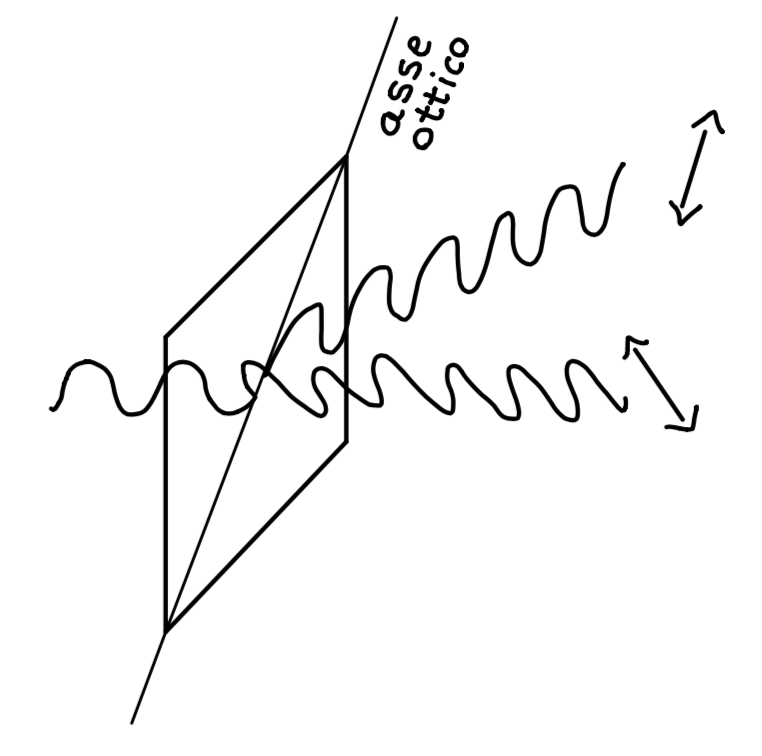
\includegraphics[width=3.5cm]{Immagini/cristallobirifrangente.png}}
È poi possibile utilizzare un cristallo di forma speculare per \q{ricomporre} i due raggi prodotti da un primo cristallo e ricostruire un'onda unica, identica - nei limiti sperimentali - a quella originaria.\\
\textbf{Setup dell'esperimento} \marginpar{Esperimento sulla polarizzazione} Lungo il cammino ottico di un fascio luminoso in luce polarizzata a $45^\circ$ rispetto a $\hat{x}$ si pongono due cristalli di calcite (birifrangenti) speculari. Il primo scompone il fascio in due raggi, di polarizzazioni $\ket{x}$ e $\ket{y}$, che vengono poi ricomposti dal secondo in un unico fascio, che infine incide contro un filtro polarizzatore tale da lasciar passare solo le onde con polarizzazione a $\ket{\minus 45^\circ}$ rispetto a $\hat{x}$.\\
Ci aspettiamo che dal filtro non passi nulla, poiché $\braket{45^\circ|\minus 45^\circ} = 0$ (la polarizzazione della luce incidente è esattamente ortogonale a quella che lascerebbe passare il filtro, quindi non passa niente), e infatti ciò si verifica sperimentalmente.\\
\begin{center}
\begin{tikzpicture}[line cap=round,line join=round,>=triangle 45,x=1.0cm,y=1.0cm,scale=0.25]
\clip(11.4985850551426,4.454563000497921) rectangle (54.015342132931025,20.40328153292733);
\draw [line width=1.2pt] (33.551209532577374,17.357389702988325)-- (30.28793239442337,19.10119750081857);
\draw [line width=1.2pt] (33.551209532577374,7.413467681243295)-- (30.28793239442337,5.669659883413049);
\draw [line width=1.2pt] (16.80335812127294,7.413467681243301)-- (20.066635259426974,5.669659883413049);
\draw [line width=1.2pt] (16.80335812127294,17.357389702988318)-- (20.066635259426974,19.10119750081857);
\draw [line width=1.2pt] (16.80335812127294,17.357389702988318)-- (16.80335812127294,7.413467681243301);
\draw [line width=1.2pt] (20.066635259426974,19.10119750081857)-- (20.066635259426974,5.669659883413049);
\draw [line width=1.2pt] (30.28793239442337,19.10119750081857)-- (30.28793239442337,5.669659883413049);
\draw [line width=1.2pt] (33.551209532577374,17.357389702988325)-- (33.551209532577374,7.413467681243295);
\draw [domain=11.4985850551426:54.015342132931025] plot(\x,{(-9.741261587570186-0.*\x)/-1.});
\draw (16.80335812127294,9.741261587570186)-- (20.066635259426974,16.);
\draw (30.28793239442337,16.)-- (33.551209532577374,9.741261587570186);
\draw (20.066635259426974,16.)-- (30.28793239442337,16.);
\draw [rotate around={90.:(43.21331647950007,9.74126158757025)},line width=1.2pt] (43.21331647950007,9.74126158757025) ellipse (4.2167323136810335cm and 1.5934904802918346cm);
\draw (23.531233397660985,12.949968214571886) node[anchor=north west] {$|x\rangle$};
\draw (23.531233397660985,19.1504761772681) node[anchor=north west] {$|y\rangle$};
\draw (11.84080394153518,12.944674979938559) node[anchor=north west] {$|45^\circ\rangle$};
\draw (36.5957681386534,17.389699221990362) node[anchor=north west] {Polarizzatore a $45^\circ$};
\draw (45.791046362053336,13.034152006008927) node[anchor=north west] {{$\langle 45^\circ | \minus 45^\circ \rangle$}};
\draw [->] (13.408244991487084,9.741261587570186) -- (14.027642058998792,9.741261587570186);
\draw [->] (24.739567814789485,16.) -- (25.249659517446183,16.);
\draw [->] (24.739567814789485,9.741261587570186) -- (25.249659517446183,9.741261587570186);
\draw [->] (36.86529988247282,9.741261587570186) -- (37.539408387331406,9.741261587570186);
\end{tikzpicture} \end{center}
Proviamo a verificarlo analiticamente. Supponiamo che ogni fotone abbia sempre una polarizzazione ben definita, che venga eventualmente modificata dalle interazioni.\\
Allora, se un raggio è in polarizzazione $\ket{y}$ il polarizzatore a $\minus 45^\circ$ ne lascia passare una frazione:
\[
\abs{\braket{y|\minus 45^\circ}}^2 = \abs{\left\langle y\bigg|\frac{1}{\sqrt{2}}(\ket{x}-\ket{y})\right\rangle}^2 = \frac{1}{2} 
\]
e analogamente $\abs{\braket{x|\minus 45^\circ}}^2 = \frac{1}{2}$.\\
Esaminiamo ora l'incidenza del fascio iniziale contro il primo cristallo. Partendo da $\ket{45^\circ}$ la probabilità di passare alla polarizzazione $\ket{x}$ è $\abs{\braket{45^\circ |x}}^2 = \frac{1}{2}$, e analogamente nel caso del passaggio a $\ket{y}$: $\abs{\braket{45^\circ|y}}^2=\frac{1}{2}$.\\
Ma se $\abs{\braket{45^\circ |x}}^2$ desse effettivamente la probabilità che il fotone sia nello stato $\ket{x}$ dopo il primo cristallo, allora la probabilità che passi il polarizzatore è:
\[
\abs{\braket{45^\circ |x}}^2 \abs{\braket{{x}|\minus 45^\circ}}^2 = \frac{1}{2}\cdot \frac{1}{2} = \frac{1}{4}
\] %sistemare \left e \right per i |
e analogamente per $\ket{y}$.\\
Se il fotone ha una polarizzazione sempre ben definita, allora tra i due cristalli essa sarà o $\ket{x}$ o $\ket{y}$, e le due possibilità sono mutualmente esclusive.
Perciò la probabilità che un fotone superi il filtro polarizzatore sarà data dalla somma delle probabilità dei possibili modi (mutualmente esclusivi) che lo portano a superarlo. Otteniamo quindi:
\[
\mathcal{P} = \frac{1}{4} + \frac{1}{4} = \frac{1}{2} \neq 0
\]
che contrasta con il risultato sperimentale.\\
Proviamo a svolgere lo stesso conto utilizzando la completezza di Dirac:\marginpar{Risultati con il formalismo di Dirac}
\begin{align*}
0 &= \abs{\bra{45^\circ} \bb{I}|\ket{\minus 45^\circ}}^2 = \abs{\braket{45^\circ|x}\braket{x|\minus 45^\circ} + \braket{45^\circ|y}\braket{y|\minus 45^\circ}}^2 =\\
&= \abs{\braket{45^\circ|x}\braket{x|\minus 45^\circ}}^2 + \abs{\braket{45^\circ|y}\braket{y|\minus 45^\circ}}^2 + \text{(termini misti)}
\end{align*}
dove i termini misti sono dati dal doppio prodotto (termine di interferenza). In questo caso, svolgendo i conti, si scopre che l'interferenza è completamente distruttiva, e ciò spiega il risultato finale.\\
Ciò significa che se non osservo il risultato intermedio tra i cristalli le alternative $\ket{x}$ e $\ket{y}$ classicamente mutualmente esclusive (sono percorsi spazialmente separati!) interferiscono tra di loro e quindi non possiamo dire che il fotone tra i cristalli abbia polarizzazione $\ket{x}$ o $\ket{y}$. Ma allora la probabilità quantistica di eventi intermedi che sono mutualmente esclusivi classicamente, se non osservati, non soddisfa la regola della probabilità classica.\\
Più precisamente, se partiamo da un insieme $I$ e andando in un insieme $\{m\}$ di alternative mutualmente esclusive che portano tutte ad uno stato $f$, classicamente la probabilità di andare da $I$ a $F$ è \[
\mathcal{P}_{I\to F} = \sum_m \mathcal{P}_{I\to m}\mathcal{P}_{m\to F}
\]
Quantisticamente, tuttavia, non si sommano le probabilità, ma le ampiezze (complesse) di probabilità, per poi calcolare il modulo quadro per ottenere la probabilità vera e propria.\\ 
La ragione per cui è possibile violare la legge di composizione delle probabilità classiche è nuovamente che \textbf{se non osserviamo la posizione del fotone, tale grandezza non assume valori}. 
\end{document}
